\begin{figure}[ht]
\tikzset{black/.style={shape=circle,draw=black,fill=black,inner sep=1pt, minimum size=9pt}}
\tikzset{white/.style={shape=circle,draw=black,fill=white,inner sep=1pt, minimum size=9pt}}

\tikzset{invisible/.style={shape=circle,draw=black,fill=black,inner sep=0pt, minimum size=0.1pt}}
\begin{center}
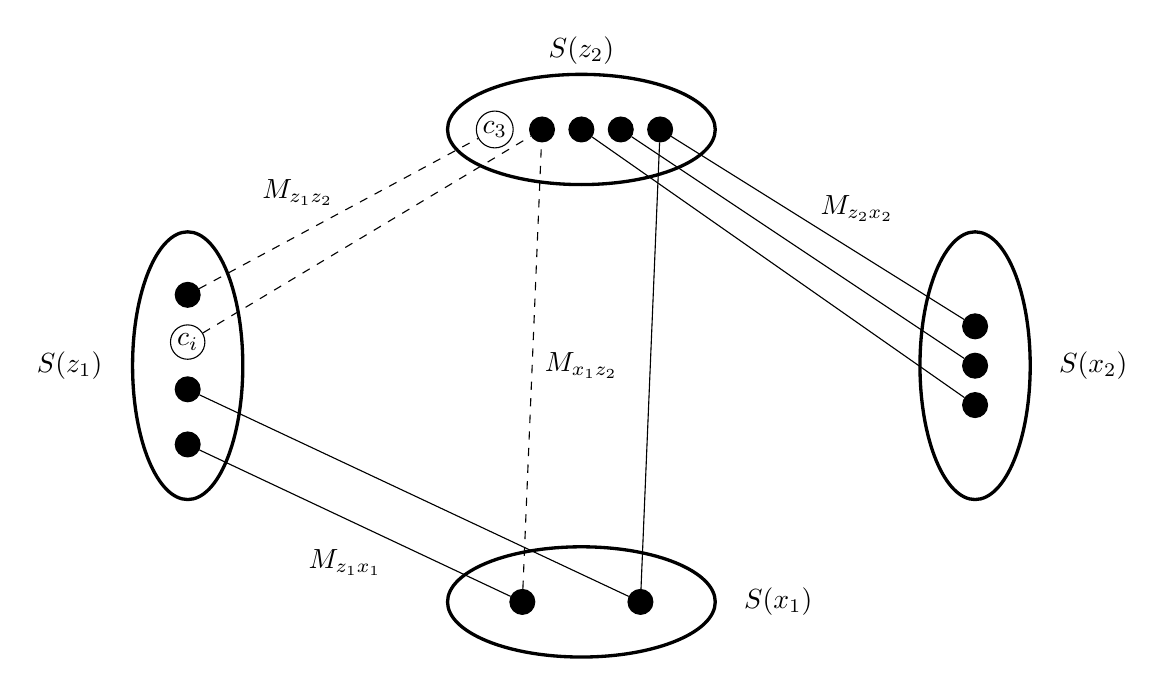
\begin{tikzpicture}
\filldraw[color=black!100, fill=black!0, very thick] (0,-3) ellipse (1.7 and 0.7);
\filldraw[color=black!100, fill=black!0, very thick] (5,0) ellipse (0.7 and 1.7);
\filldraw[color=black!100, fill=black!0, very thick] (-5,0) ellipse (0.7 and 1.7);
\filldraw[color=black!100, fill=black!0, very thick] (0,3) ellipse (1.7 and 0.7);
        \node[] at (-6.5,0) {$S(z_1)$};
        \node[] at (2.5,-3) {$S(x_1)$};
        \node[] at (6.5,0) {$S(x_2)$};
        \node[] at (0,4) {$S(z_2)$};
        
        \node[] at (0,0) {$M_{x_1z_2}$};
        \node[] at (-3.6,2.2) {$M_{z_1z_2}$};
        \node[] at (3.5,2) {$M_{z_2x_2}$};
        \node[] at (-3,-2.5) {$M_{z_1x_1}$};

        \node[black] (1) at (-5,0.9){};
        \node[white] (2) at (-5,0.3){$c_i$};
        \node[black] (3) at (-5,-0.3){};
        \node[black] (4) at (-5,-1){};
        \node[black] (5) at (-0.75,-3){};
        \node[black] (6) at (0.75,-3){};
        \node[black] (7) at (5,-0.5){};
        \node[black] (8) at (5,0){};
        \node[black] (9) at (5,0.5){};
        \node[black] (10) at (1,3){};
        \node[black] (11) at (0.5,3){};
        \node[black] (12) at (0,3){};
        \node[black] (13) at (-0.5,3){};
        \node[white] (14) at (-1.1,3){$c_3$};

        \draw[black] (3)--(6); 
        \draw[black] (4)--(5); 
        \draw[black] (6)--(10); 
        \draw[black] (9)--(10); 
        \draw[black] (8)--(11); 
        \draw[black] (7)--(12); 
        \draw[dashed] (5)--(13);
        \draw[dashed] (2)--(13);
        \draw[dashed] (1)--(14);

\end{tikzpicture}


\caption{The matchings between $S(x_1)$, $S(x_2)$, $S(z_1)$, and $S(z_2)$, as described in Claim \ref{keyclaim}. The matching $M_{x_2x_1}$ is omitted for clarity. We assume there exists a colour $d_1 \in S(x_1)$ and $d_2 \in S(x_2)$ such that $z_2[x_1,d_1] = z_2[x_2,d_2]$. Without loss of generality, we may assume that the solid edges in the matchings are as shown. No matter the remainder of the edges in $M_{z_1z_2}$ and $M_{x_1z_2}$, there exist colours $c_i \in S(z_1)$ and $c_3 \in S(z_2)$ such that $c_i$ is unmatched in $M_{x_1z_1}$, such that $c_3$ is unmatched in $M_{x_1z_2}$ and $M_{x_2z_2}$, and such that $c_3 \neq z_2[z_1, c_i]$.} 
    \label{fig:matchings1}
\end{center}
\end{figure}






